\subsubsection{Gestão de fases e entregas}

Na página dedicada à gestão de fases e entregas, um aluno pode consultar todas as informações das fases de um projeto, todas as entregas relativas às referidas fases e pode submeter novas entregas para a fase atual.

Sendo a submissão de entregas um dos processos mais críticos do sistema, pretende garantir-se a partir desta página mais flexibilidade e segurança para aluno ao longo deste processo.\\

Relativamente às fases, num plano principal, são apresentadas informações relativas às datas de inicio e de fim da fase, descrição, ficheiros de entrega obrigatória, ficheiros auxiliares, e atalhos para a pauta e para o enunciado da fase.

São ainda listadas todas as entregas para a referida fase.

Para cada entrega, o utilizador pode fazer \textit{download} de todos os ficheiros entregues como um ficheiro \textit{ZIP}.\\

Num painel mais à direita pode encontrar-se o formulário de submissão de nova entrega.

Esse formulário apenas será mostrado ao utilizador se forem verificadas duas restrições, pertencer a um grupo válido, e existir no momento uma fase ativa.

É importante referir que para uma submissão mais cómoda de ficheiros grandes, o utilizador pode carregar os ficheiros antes de proceder à submissão da entrega.

Optou-se por simplificar ao máximo o formulário de submissão de nova entrega, assim sendo, o utilizador apenas necessita de colocar os ficheiros e uma descrição da entrega.\\

Na Figura~\ref{fig:student_deliveries} pode ser consultada uma imagem demonstrativa da página desenvolvida.

\begin{figure}[H]
  \centering
  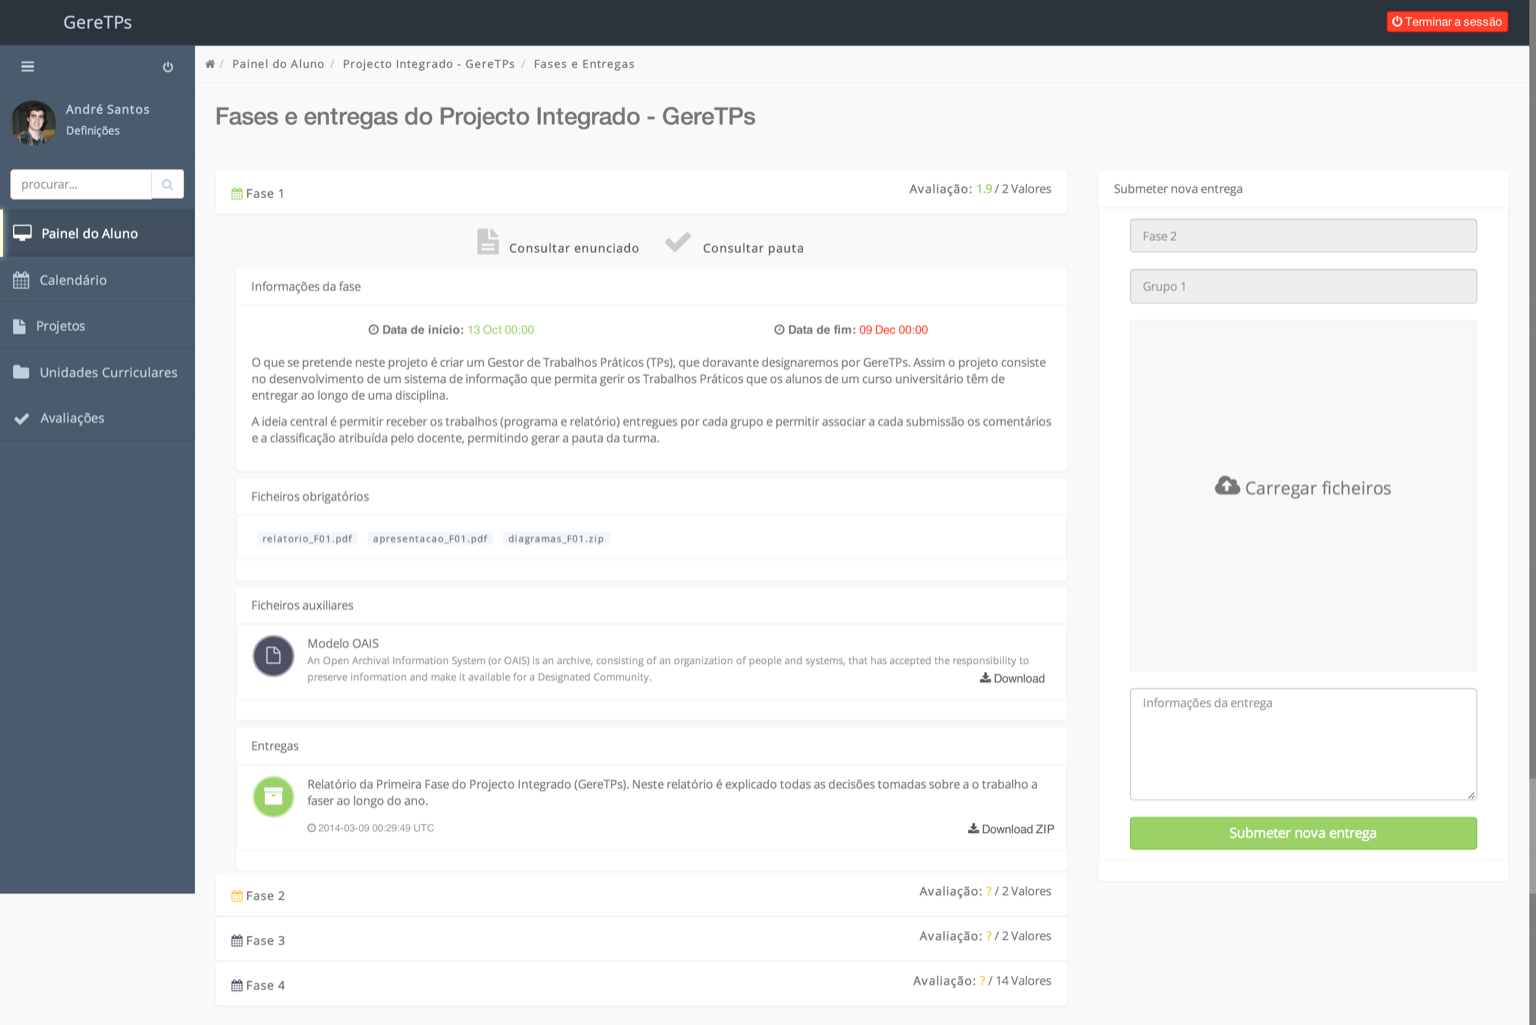
\includegraphics[width=1\textwidth,center]{images/implementacao/alunos/deliveries}
  \caption{Página de gestão de fases entregas}
  \label{fig:student_deliveries}
\end{figure}
